\section{EXPERIMENT}
In this section, we first describe the testbed and then present the results of the experiments.

\subsection{Testbed}

\begin{figure}[t]
  \centering
  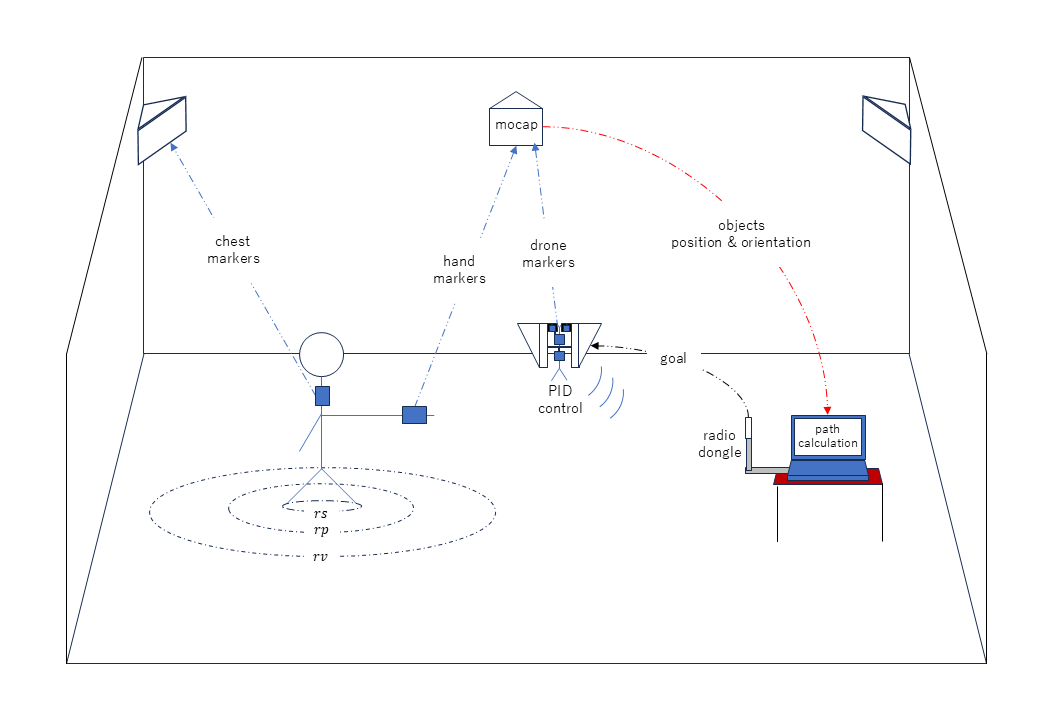
\includegraphics[width=\columnwidth]{system-chart.png}
  \caption{Overall system configuration.}
  \label{fig:system}
\end{figure}
Fig.~\ref{fig:system} illustrates the overall system configuration.
The system consists of a motion capture (MoCap) system, a flapping-wing drone, a user wearing devices, and a PC for trajectory planning and control.
The MoCap system tracks the 3D positions and orientations of the user's chest, palm, and the drone in real time.
We use eight Optitrack Prime 13 cameras on the four corners and four sides of the room.  
The user wears chest-mounted and wrist-mounted markers allowing the system to capture intuitive control gestures. 
The PC processes the positional data and calculates the drone's optimal approach path toward the user's palm while maintaining a safe distance. 
The computed path is transmitted to the drone via a radio dongle, ensuring real-time control. 
The drone moves to the newest goal sent by the PC using control in Section~\ref{sec:modeling}, 
adjusting its motion dynamically based on the feedback from the MoCap system.

Then, we describe the drone used in the experiment and the interface for control in detail.
\begin{figure}[b]
  \centering
  \begin{tabular}{cc}
      \begin{minipage}[t]{0.4 \columnwidth}
        \centering
        \includegraphics[keepaspectratio, scale=0.09]{flapper.jpg}
        \subcaption{}
        \label{fig:flapper}
      \end{minipage} &
      \begin{minipage}[t]{0.4 \columnwidth}
        \centering
        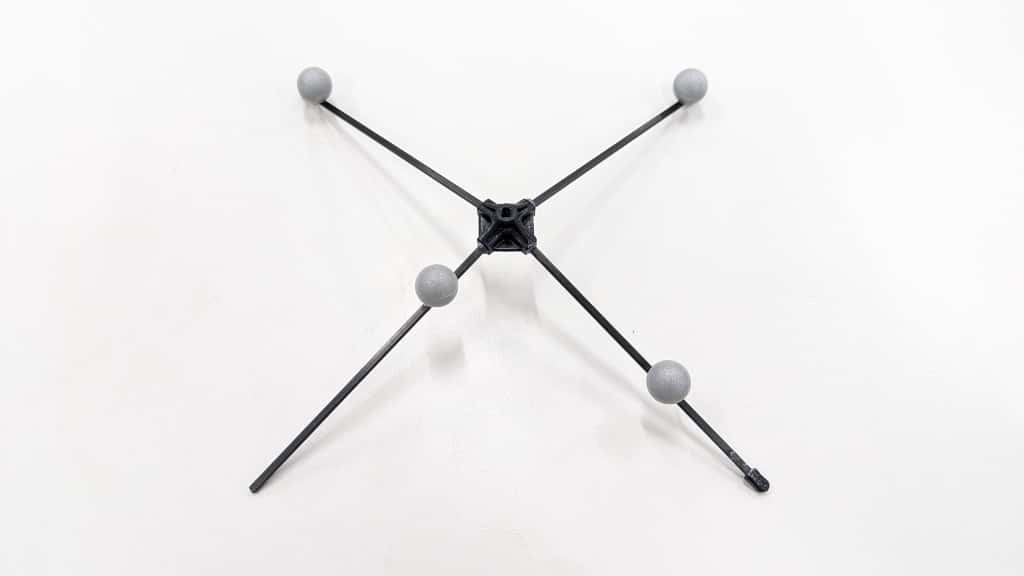
\includegraphics[keepaspectratio, scale=0.09]{leg.jpg}
        \subcaption{}
        \label{fig:leg}
      \end{minipage}
    \end{tabular}
  \caption{(a) Flapper Nimble+ drone, (b) its leg with motion capture markers.}
\end{figure}
Flapper Nimble+ \cite{company_product} used in the experiment, shown in Fig.~\ref{fig:flapper}, is a flapping-wing drone by FLAPPER DRONES compatible with the Crazyflie software, 
which is a open-source platform for research and development of quadcopters produced by Bitcraze AB. 
As shown in Fig.~\ref{fig:leg}, we attached four motion capture markers on its legs for tracking the position and orientation. 
As noted in Section~\ref{sec:motion-planning}-\ref{fig:trajectory}, the drone has to change its behavior according to the position of the user's palm.
\begin{figure}[t]
  \centering
  \begin{tabular}{cc}
      \begin{minipage}[t]{0.4 \columnwidth}
        \centering
        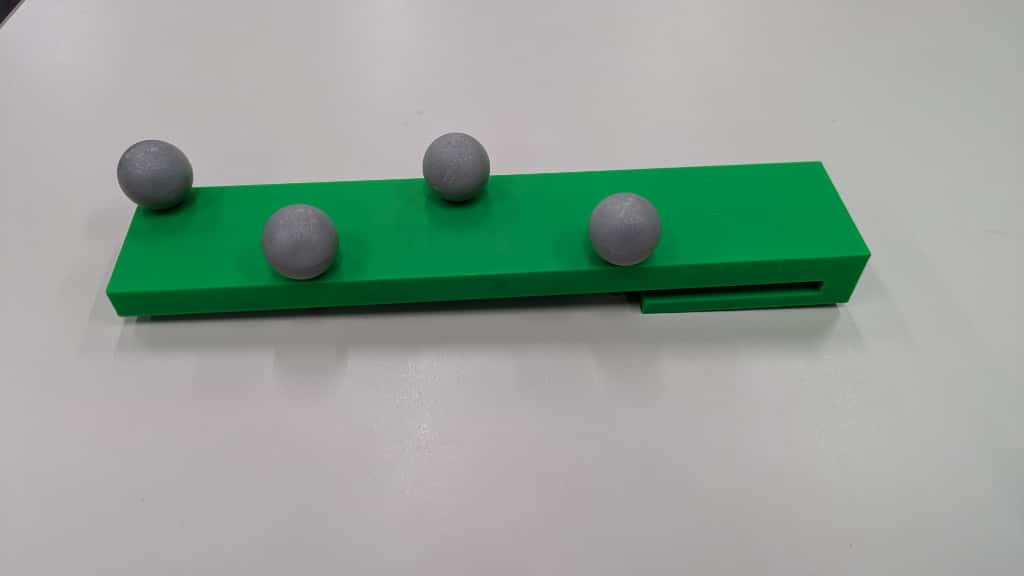
\includegraphics[keepaspectratio, scale=0.09]{chest.jpg}
        \subcaption{}
        \label{fig:chest}
      \end{minipage} &
      \begin{minipage}[t]{0.4 \columnwidth}
        \centering
        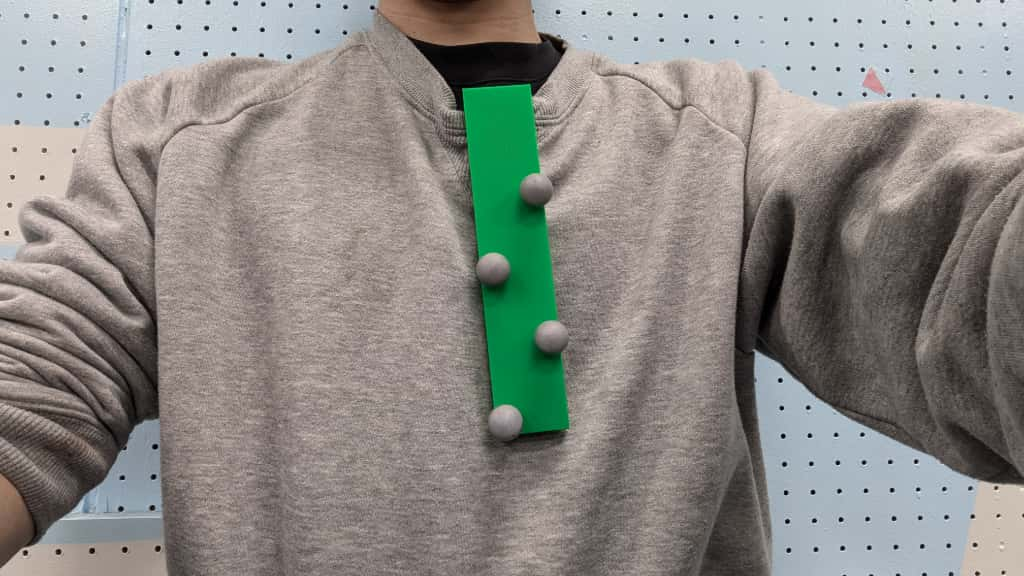
\includegraphics[keepaspectratio, scale=0.09]{chest_attach.jpg}
        \subcaption{}
        \label{fig:chest_attach}
      \end{minipage} \\
      \begin{minipage}[t]{0.4 \columnwidth}
        \centering
        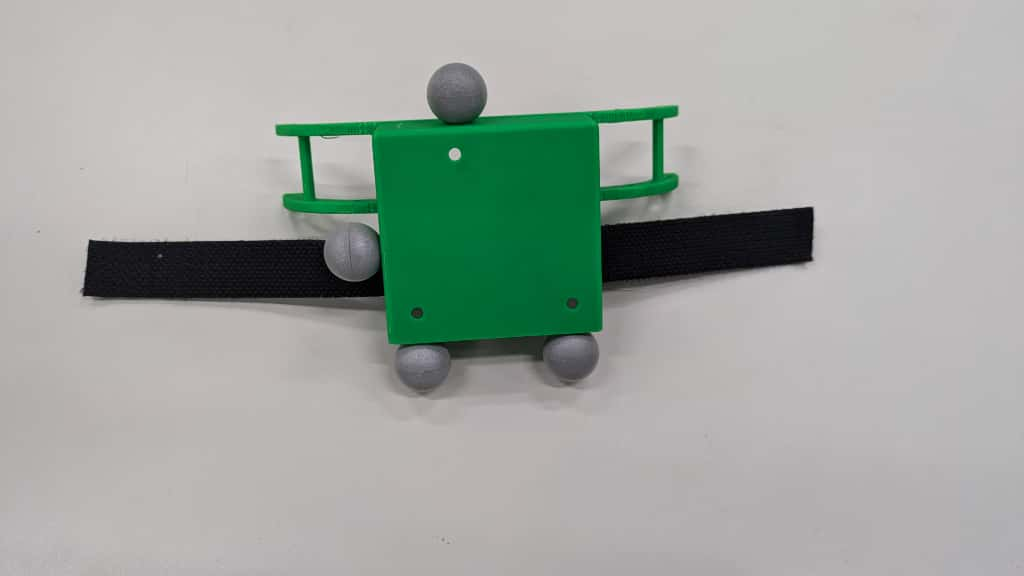
\includegraphics[keepaspectratio, scale=0.09]{hand.jpg}
        \subcaption{}
        \label{fig:hand}
      \end{minipage} &
      \begin{minipage}[t]{0.4 \columnwidth}
        \centering
        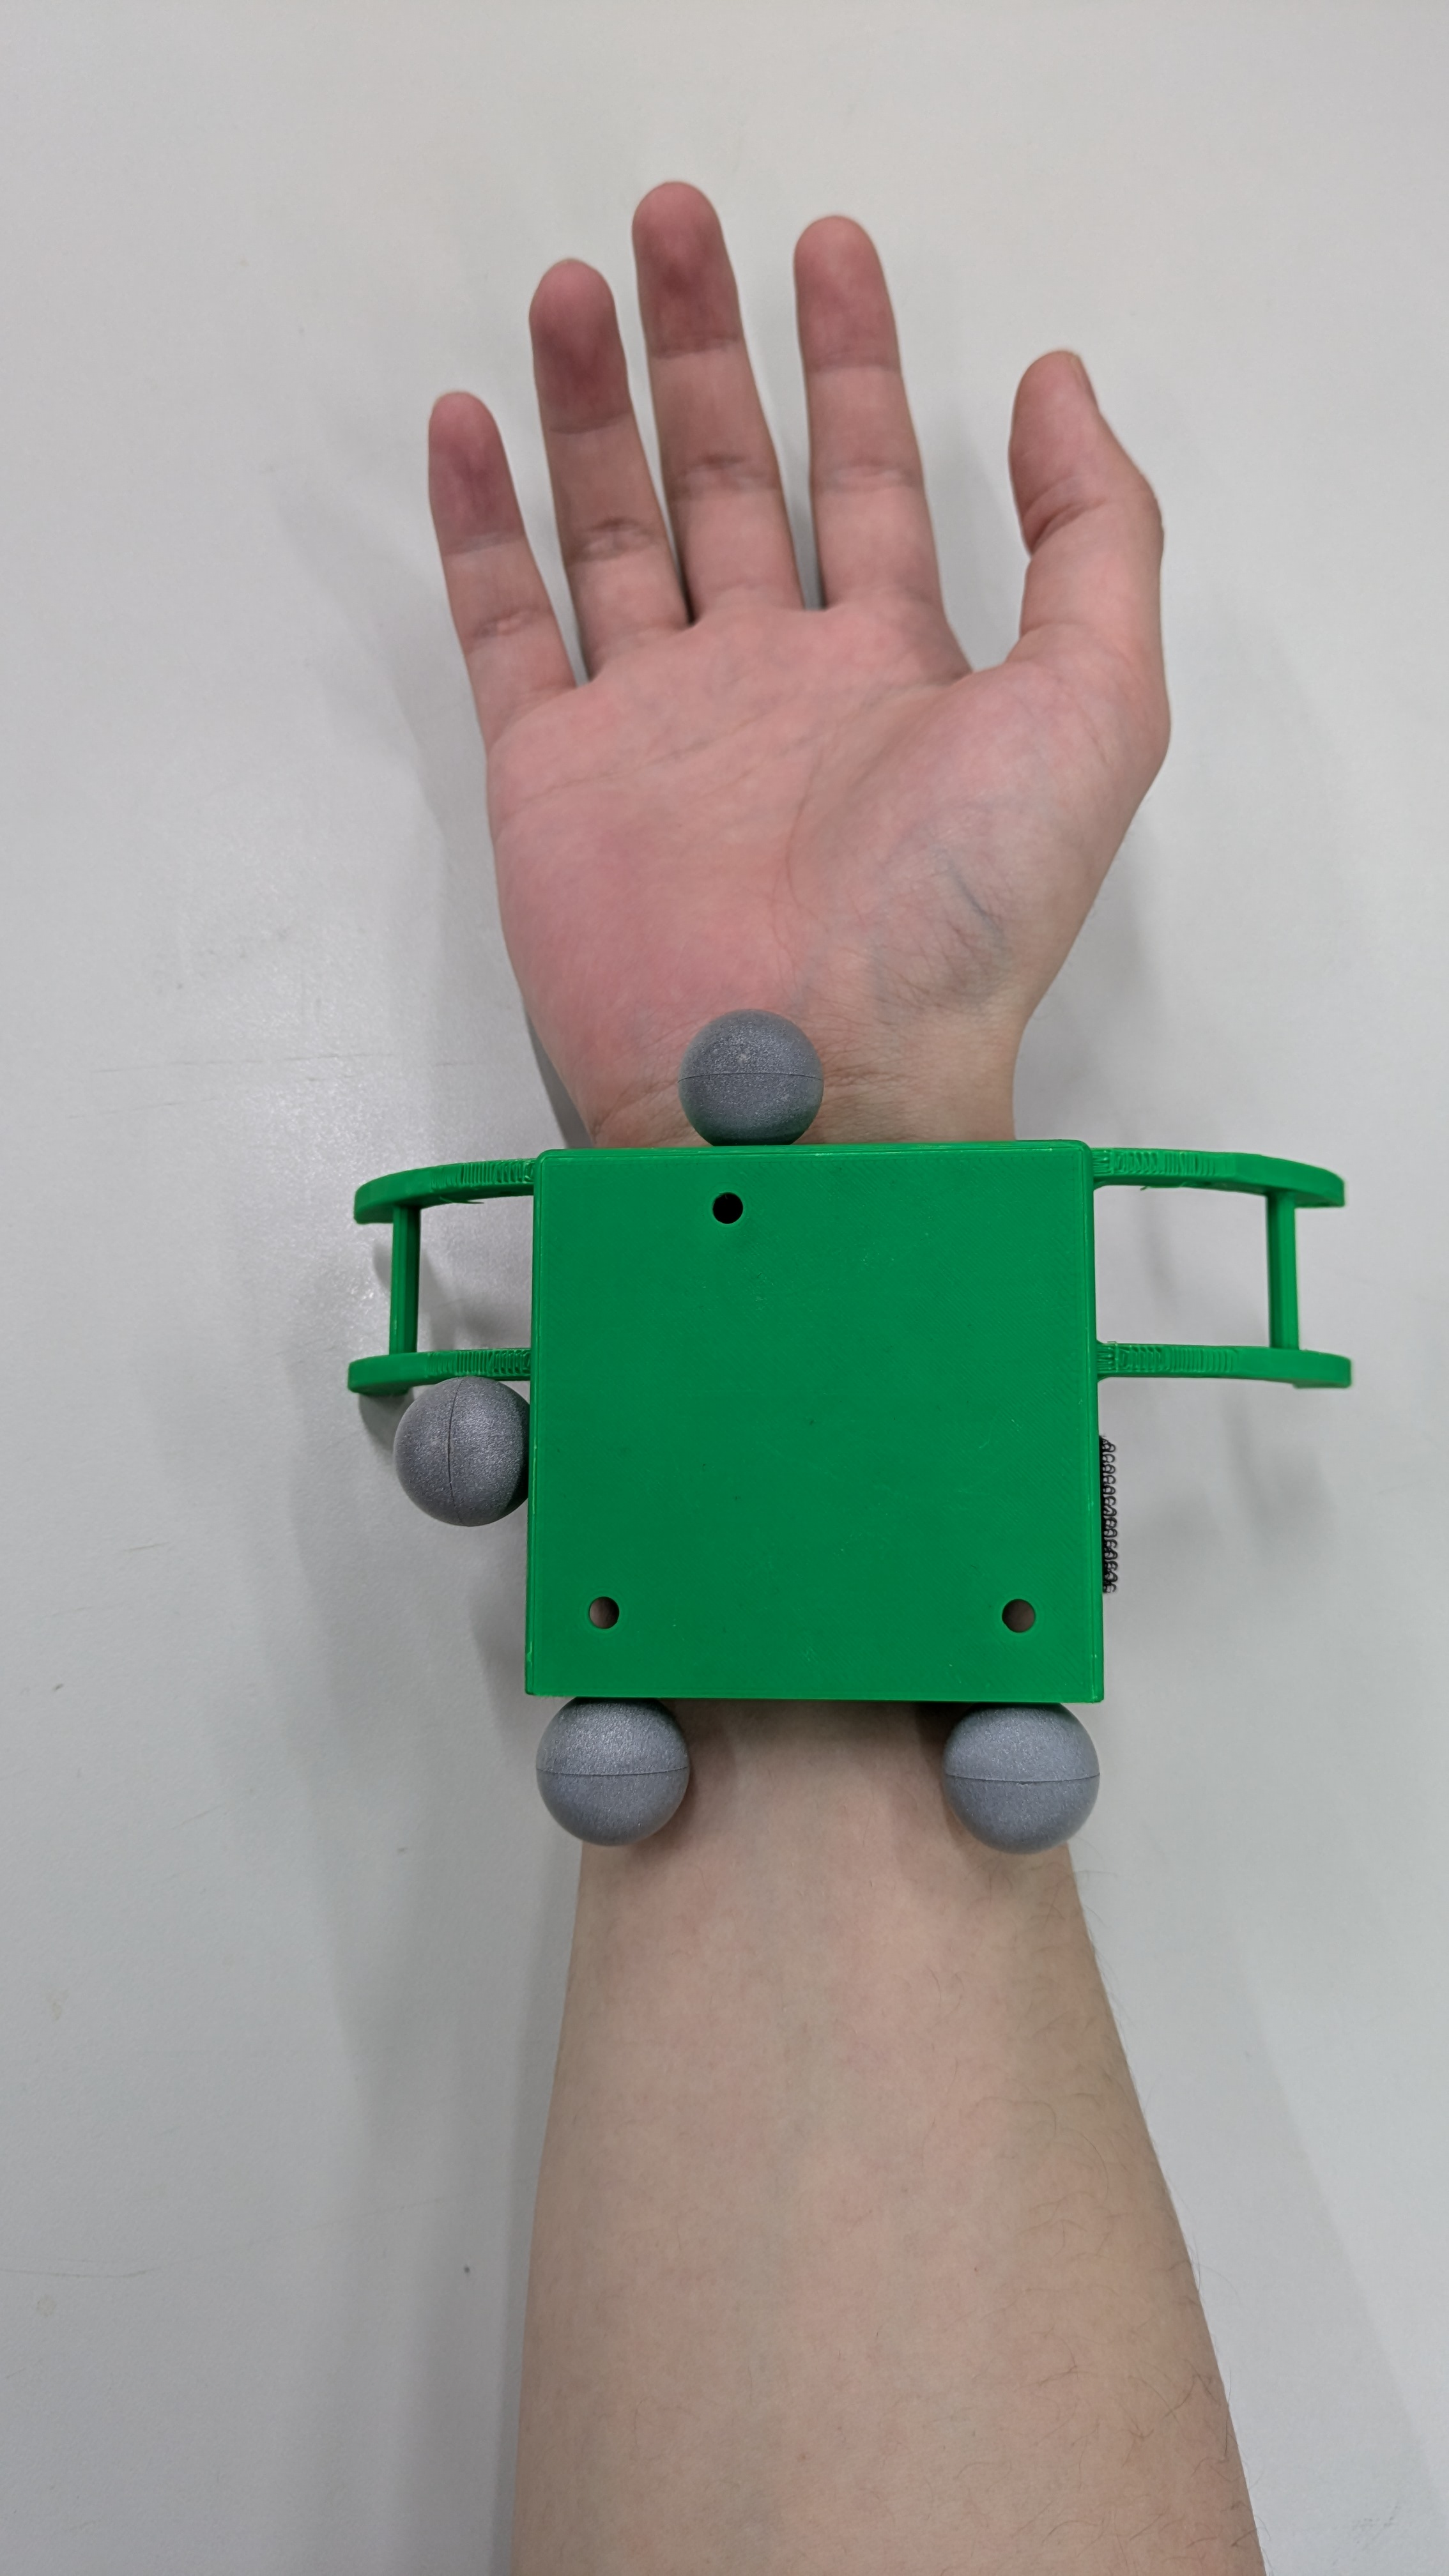
\includegraphics[keepaspectratio, scale=0.051, angle=90]{hand_attach.jpg}
        \subcaption{}
        \label{fig:hand_attach}
      \end{minipage}
    \end{tabular}
  \caption{(a) Chest-mounted device, (c) wrist-mounted device for controlling the state of flapping drone. (b, d) the attachment of the devices.}
\end{figure}
To facilitate intuitive control, we designed a wearable interface consisting of 
a chest-mounted device shown in Fig.~\ref{fig:chest} and 
a wrist-mounted device shown in Fig.~\ref{fig:hand}.
Both devices were fabricated using a PLA 3D printer. 
With these devices, we acquired the user's palm position and orientation from the motion capture system and calculate the desired drone behavior based on the user's palm position. 
This interaction design only requires arm bending and stretching to switch the state of the drone and thus enables a seamless and intuitive approach control.
\subsection{Palm Landing Experiments}
\begin{figure}[b]
    \begin{tabular}{cc}
      \centering
      \begin{minipage}[t]{0.45 \columnwidth}
        \centering
        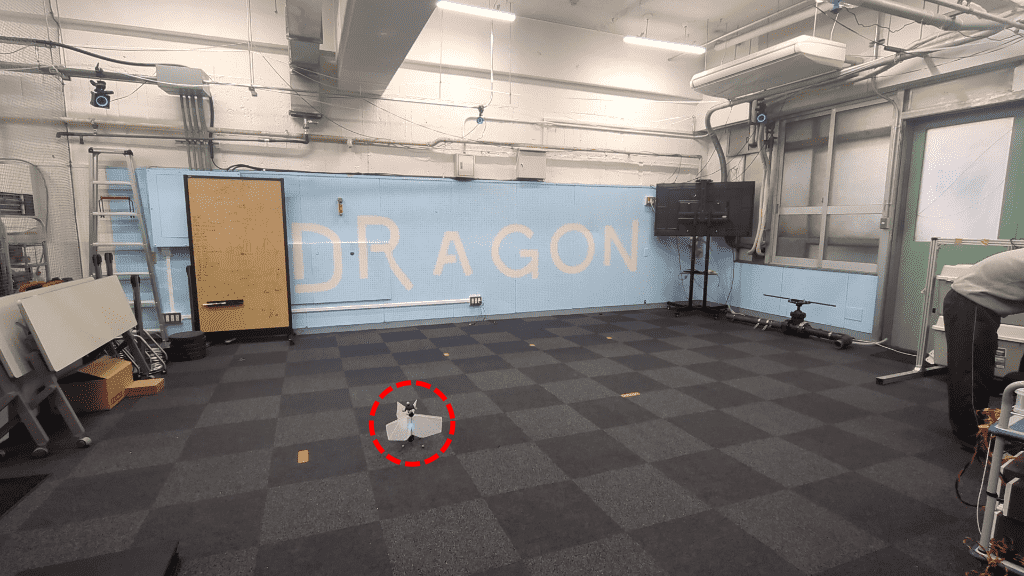
\includegraphics[keepaspectratio, scale=0.09]{start.png}
        \subcaption{}
        \label{fig:start}
      \end{minipage}&
      \begin{minipage}[t]{0.45 \columnwidth}
        \centering
        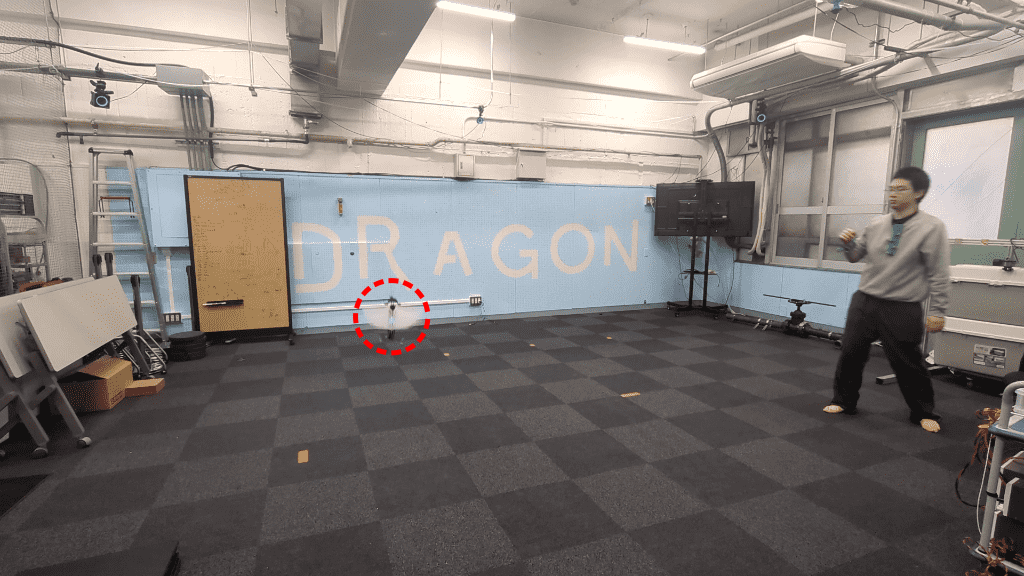
\includegraphics[keepaspectratio, scale=0.09]{takeoff.png}
        \subcaption{}
        \label{fig:takeoff}
      \end{minipage} \\
      \begin{minipage}[t]{0.45 \columnwidth}
        \centering
        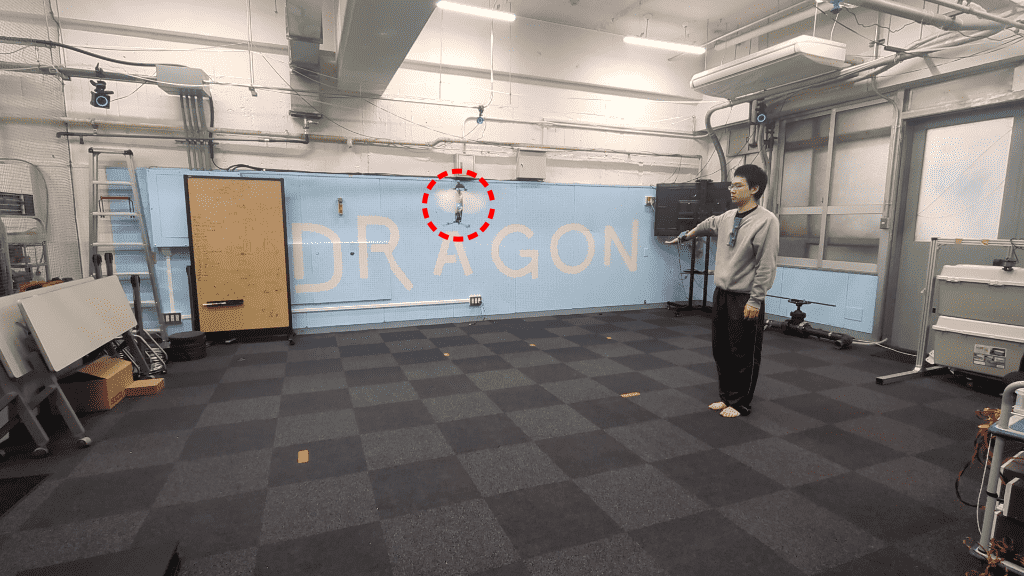
\includegraphics[keepaspectratio, scale=0.09]{approach.png}
        \subcaption{}
        \label{fig:approach}
      \end{minipage}&
      \begin{minipage}[t]{0.45 \columnwidth}
        \centering
        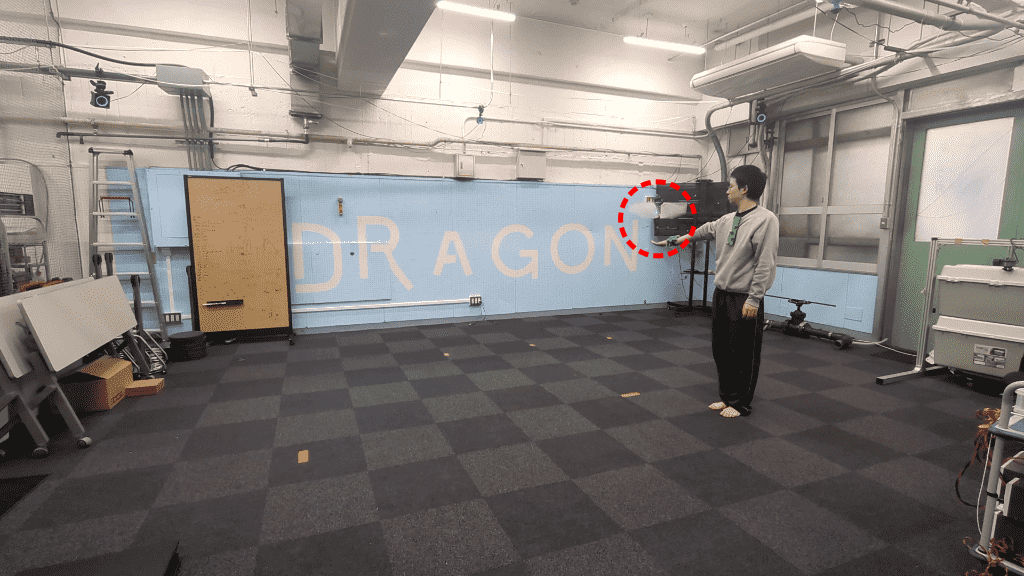
\includegraphics[keepaspectratio, scale=0.09]{palm-land.png}
        \subcaption{}
        \label{fig:palm-land}
      \end{minipage}      
    \end{tabular}
    \caption{The drone states during the experiment. (a) Start, (b) Takeoff, (c) Approach, (d) Palm landing.}
    \label{fig:states}
\end{figure}
\begin{figure}[t]
  \centering
  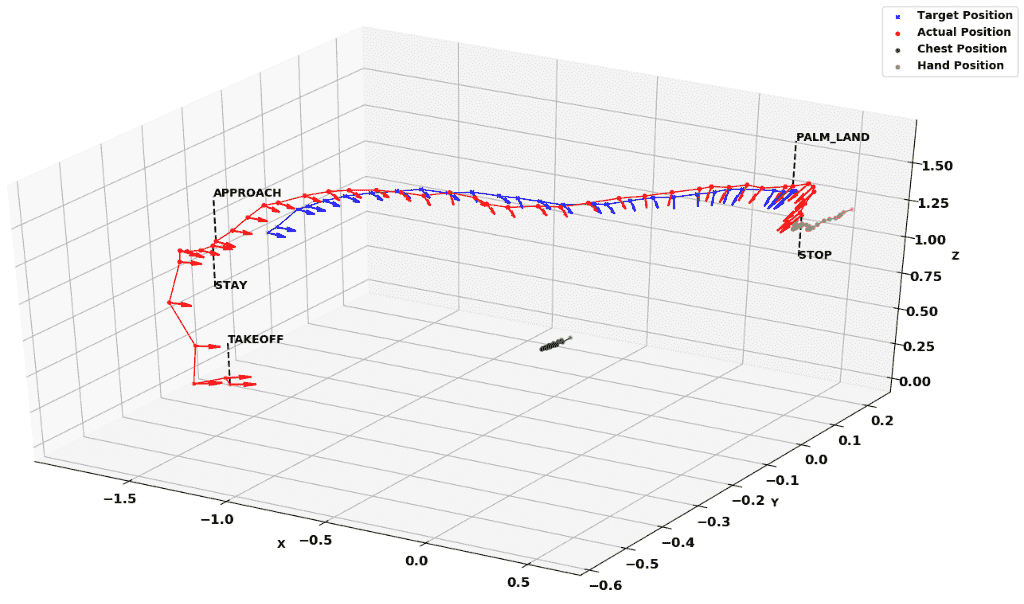
\includegraphics[keepaspectratio, scale=0.23]{simple-hand-landing-trajectory.png}
  \caption{Trajectory and orientations of the drone during the approach.
  The red points indicates the actual positions of the drone during the approach and the blue points the target positions. 
  The arrows extruding from the red points indicate the orientation of the drone.
  The blue points show when the drone reaches "APPROACH" state.}
  \label{fig:simple_hand_landing_trajectory}
\end{figure}
Fig.~\ref{fig:states} shows the drone states during the experiment.
We explain the results of the experiment in the following sections.

\subsubsection{Trajectory Mapping}
In Fig.~\ref{fig:simple_hand_landing_trajectory}, it can be observed that the drone closely followed the planned trajectory and the drone's orientation always faced the user's chest.
We calculated the root mean square error (RMSE) between the actual and target positions of the drone, which was 0.1695m.
Additionally, the drone's actual position was approximately 1.0s behind the target position,
which is about ten times larger than the time interval $\Delta t$ of 0.1s.
This suggests that the drone's response time was significantly slower than expected from (\ref{eq:goal}).
This delay is considered to be due to the delay in the control system.
The delay means that the drone's actual speed is slower than the calculated speed in (\ref{eq:speed}), which can be overly safe for the user and make the user feel irritated.

\begin{figure}
  \centering
  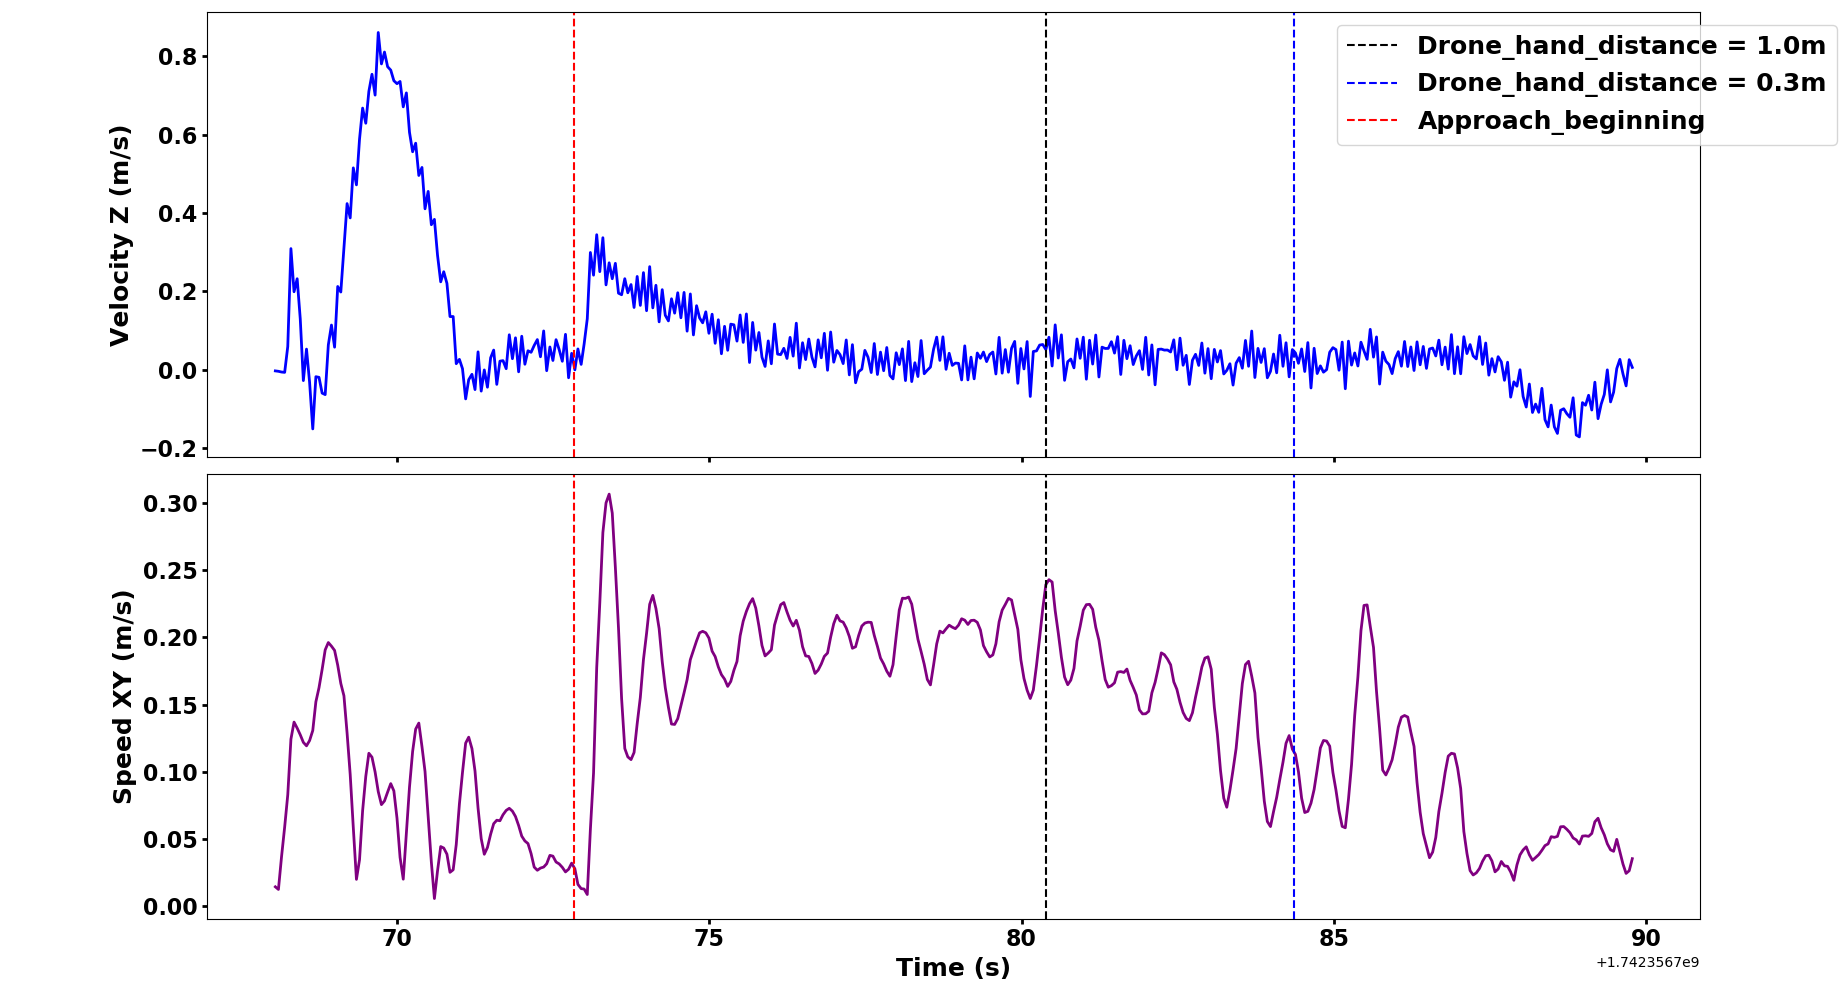
\includegraphics[keepaspectratio, scale=0.18]{simple-hand-landing-vel.png}
  \caption{Velocity of the drone during the approach. 
  The vertical dotted red line indicates the approach start time, 
  the black line the time when the drone starts to decelerate, 
  and the blue line the time when $k^\prime$ changes from 0.2 to 0.5.}
  \label{fig:simple_hand_landing_vel}
\end{figure}
\subsubsection{Velocity}
In Fig.~\ref{fig:simple_hand_landing_vel},
it is observed that between the red and black lines, the purple plot oscillated around a constant value, and between the black and blue lines, the XY speed decreased with oscillation.
The oscillation is considered to be due to the constantly updated goal position at a certain frequency.
From (\ref{eq:weber}), the oscillation causes instability in $\Delta s$,
which causes a potential psychological threat to the user.
To mitigate this, we can consider increasing the frequency of updating the goal position or using a smoother trajectory planning method.
Additionally, in practical applications, we found that the drone became too slow at a short distance from the user due to the small $k^\prime$.
To avoid this, we changed $k^\prime$ from 0.2 to 0.5 at a distance of 0.3m from the palm.
This change can be observed in Fig.~\ref{fig:simple_hand_landing_vel} as the sudden increase in XY speed right after the blue line.

\begin{figure}
  \centering
  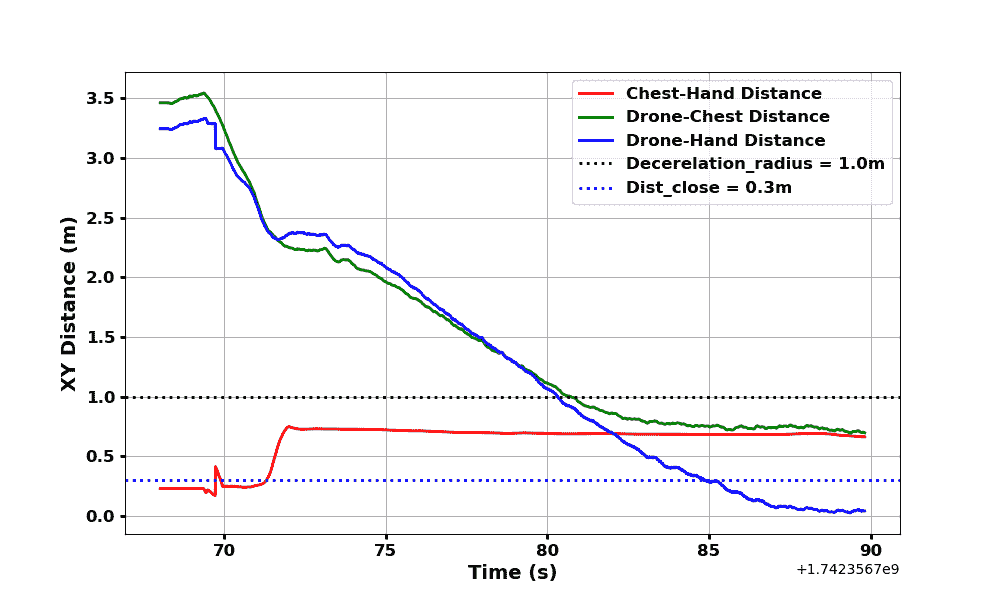
\includegraphics[keepaspectratio, scale=0.24]{XY_distances.png}
  \caption{Distance between the user's chest and the drone during the approach.}
  \label{fig:simple_hand_landing_xy_distances}
\end{figure}
\subsubsection{Distance Between Chest and Drone}
As shown in Fig.~\ref{fig:simple_hand_landing_xy_distances}, the chest-drone distance and the drone-hand distance started decreasing 
when the chest-hand distance was above 0.3m.
The minimum distance between the drone and the user's chest was 0.693m.
The drone successfully kept out of the chest-hand range.
Furthermore, the drone-hand distance gradually and smoothly decreased to zero without any overshoots,
which enabled smooth and safe palm-landing.

\subsection{Tracking Performance}
\begin{figure}
  \centering
  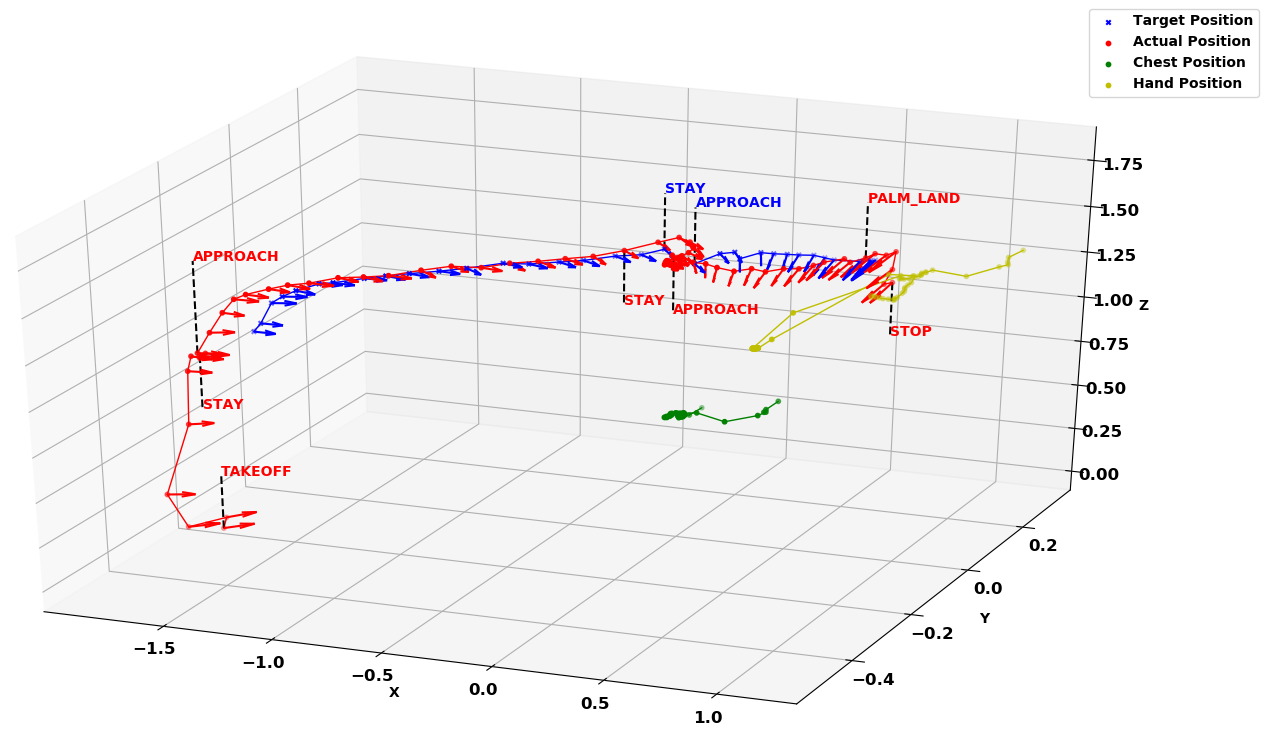
\includegraphics[keepaspectratio, scale=0.19]{switch-trajectory.png}
  \caption{Trajectory and orientations of the drone in the case of switching the drone state between "STAY" and "APPROACH".}
  \label{fig:switch}
\end{figure}
\begin{figure}
  \centering
  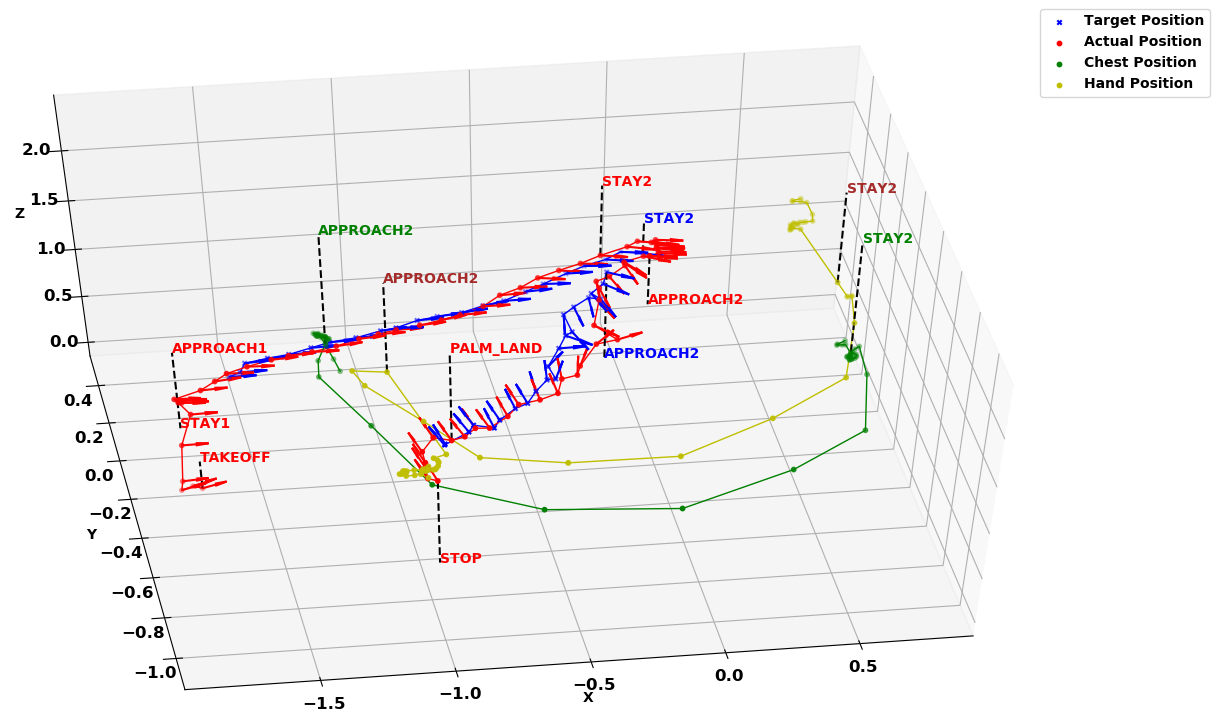
\includegraphics[keepaspectratio, scale=0.19]{moving-around-trajectory.png}
  \caption{Trajectory and orientations of the drone in the case of the user moving around. 
  The numbers after "APPROACH" and "STAY" indicate the order of the state. 
  The same labels indicate that the points are at the same time. The user moved around the drone between the state "STAY2" and "APPROACH2".}
  \label{fig:moving}
\end{figure}
As shown in Fig.~\ref{fig:switch}, the drone successfully switched between the "STAY" and "APPROACH" states,
and when the drone was in the "STAY" state, the drone maintained its current position.
However, it can be observed that right after the state switch, the drone went slightly over the target position and then swung back to the target position.
This overshoot is considered to be due to the inertia of the drone.
This type of unexpected behavior can cause threat to the user's psychological safety.
To mitigate this, we can consider adding a function to gradually decrease the drone's speed when switching the state by anticipating the change of the user's gesture.
The change of the user's gesture can be detected by the change of the chest-hand distance.
Additionally, as shown in Fig.~\ref{fig:moving}, the drone successfully followed the user's movement.
This ensures that the user can freely decide the palm-landing position and time.

